\documentclass[12pt,a4paper]{article}
\usepackage[dutch]{babel}
\usepackage[utf8]{inputenc}
\usepackage[margin=0.5in]{geometry}
\usepackage{amsmath}
\usepackage{amsfonts}
\usepackage{amssymb}
\usepackage{graphicx}
\usepackage{listings}
\usepackage{float}


\begin{document}
\graphicspath{ {./images/} }
\DeclareGraphicsExtensions{.pdf,.png,.jpg}
\lstset{language=bash}      
\author{Steven L. Speek}
\title{GNUAmsterdam Debian Wheezy Installatie}
\date{\today}
\maketitle
\abstract{Nederlandse handleiding voor een Debian desktop installatie.}


\section{Algemene aanwijzingen}
\emph{Zeer belangrijk:} Iedere vraag die door het installatie programma aan jou wordt gesteld en waarover hieronder niets staat vermeldt beantwoordt je met de \textsc{enter}-toets.

Als de debian installer naar een nieuw scherm gaat, begint er in deze handleiding een nieuwe paragraaf


\section{Floppy station onklaar maken}
Floppy stations zijn een erfenis uit het verleden. Schakel de floppy ondersteuning in de BIOS uit. En maak de kabels verbonden met het floppy-station los.


\section{CDROM ophalen}
Op \texttt{www.debian.org/distrib/}, kies je een klein installatie-image voor jouw architectuur (meestal amd64, soms nog i686).
Brandt dit op een CDROM, dit zullen wij de installatie CDROM noemen.


\section{Installatie basissysteem}
Wij gaan nu met de debian installer een simpel basissysteem installeren. Dit begint met het instellen van gegevens over onze plek op aarde en de taal die wij wensen te gebruiken met het nieuwe systeem.

Boot van de installatie CDROM. Je komt dan in een menu.
Je accepteert de eerste optie \textbf{Install} met \textsc{enter}.


\subsection{Localisatie instellingen}
\begin{figure}[H]
\centering
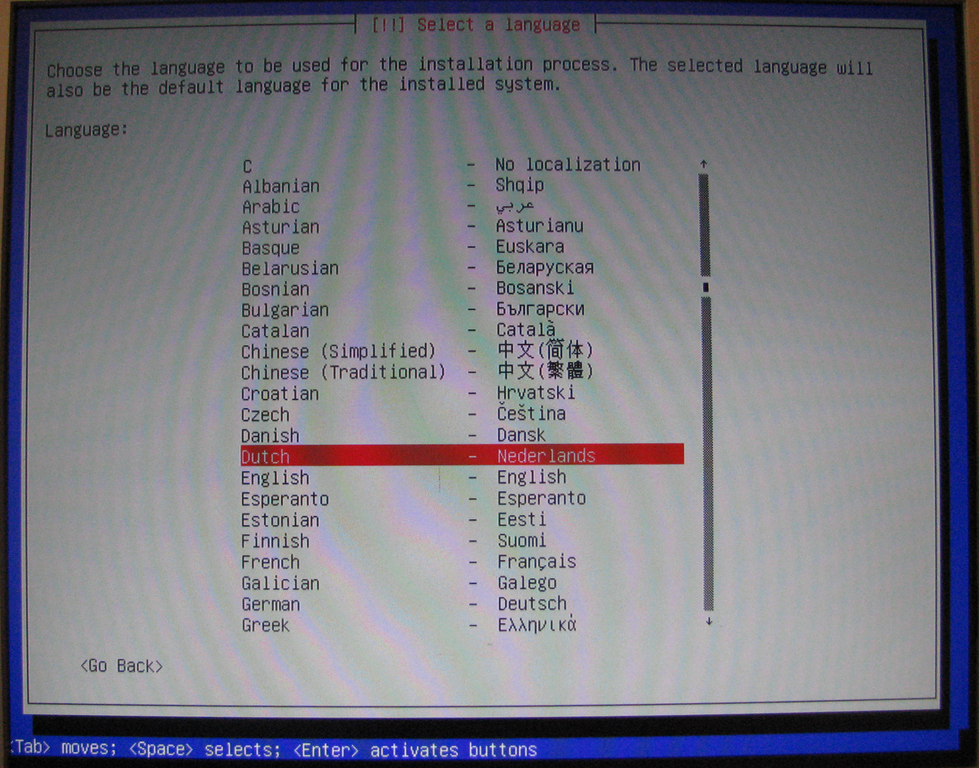
\includegraphics[width=0.45\textwidth]{taal-keuze-scherm}
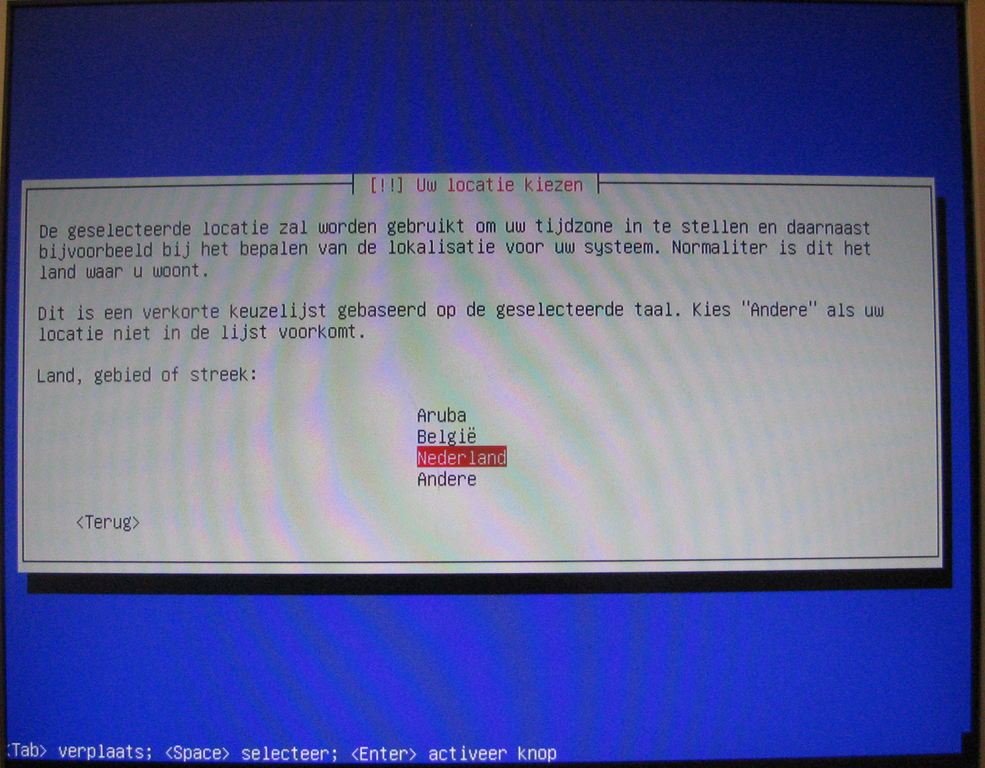
\includegraphics[width=0.45\textwidth]{lokatie-keuze-scherm}
\caption{Taal en lokatie instellingen.}
\label{fig:taal-keuze-scherm}
\end{figure}

Op het volgende twee schermen, zie figuur ~\ref{fig:taal-keuze-scherm},  moet je de taal kiezen; kies \textbf{Dutch} (pijltje omhoog en dan \textsc{enter}). In de scherm daarna, selecteer je  \textbf{Nederland} als land en drukt op \textsc{enter}. Vanaf gaan we niet meer zeggen dat je op \textsc{enter} moet drukken.

\begin{figure}[H]
\centering
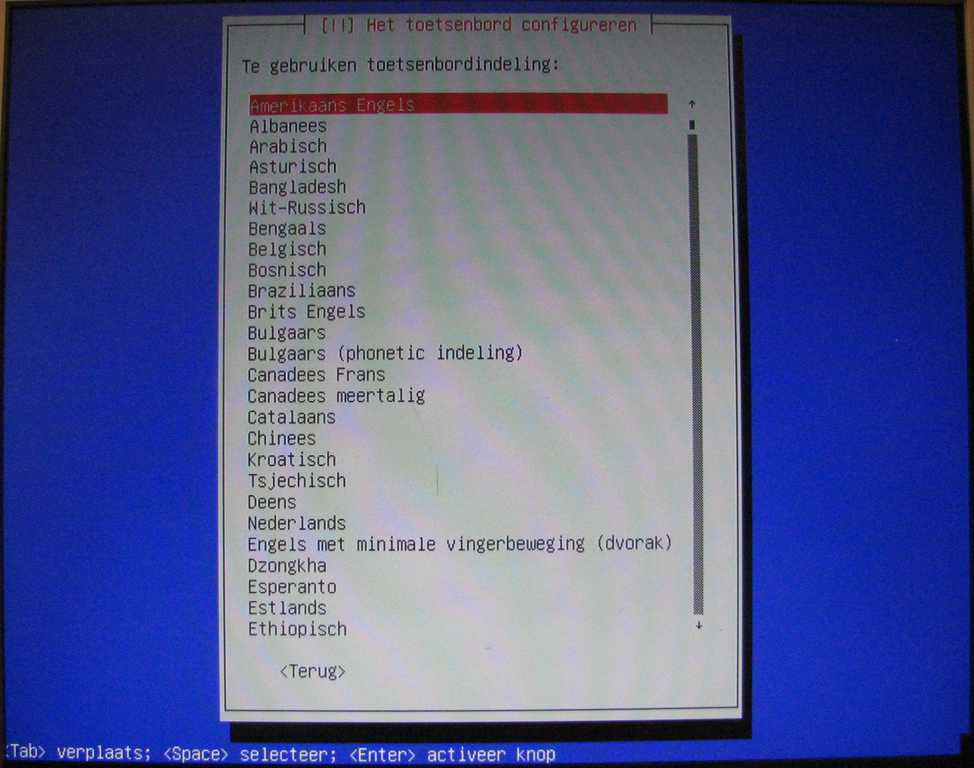
\includegraphics[width=0.45\textwidth]{toetsenbord-indeling-scherm}
\caption{Kies hier \textbf{American English}.}
\label{fig:toetsenbord-indeling-scherm}
\end{figure}

Als toetsenbordindeling kies je \textbf{American English} (zie figuur ~\ref{fig:toetsenbord-indeling-scherm}).


\subsection{Netwerk instellingen}
Je wacht tot de debian installer de aanvullende installatie modules heeft geladen. Het kan zijn dat er vragen komen over ontbrekende firmware. Die moet je allen met \textbf{nee} beantwoorden.

\begin{figure}[H]
\centering
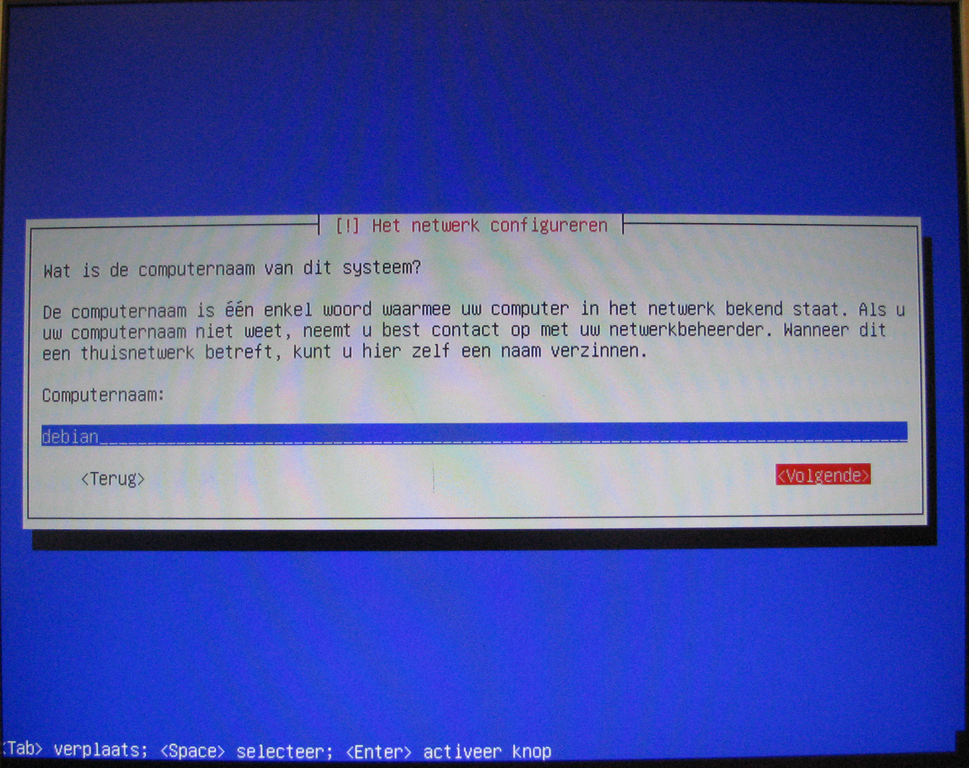
\includegraphics[width=0.45\textwidth]{computernaam-scherm}
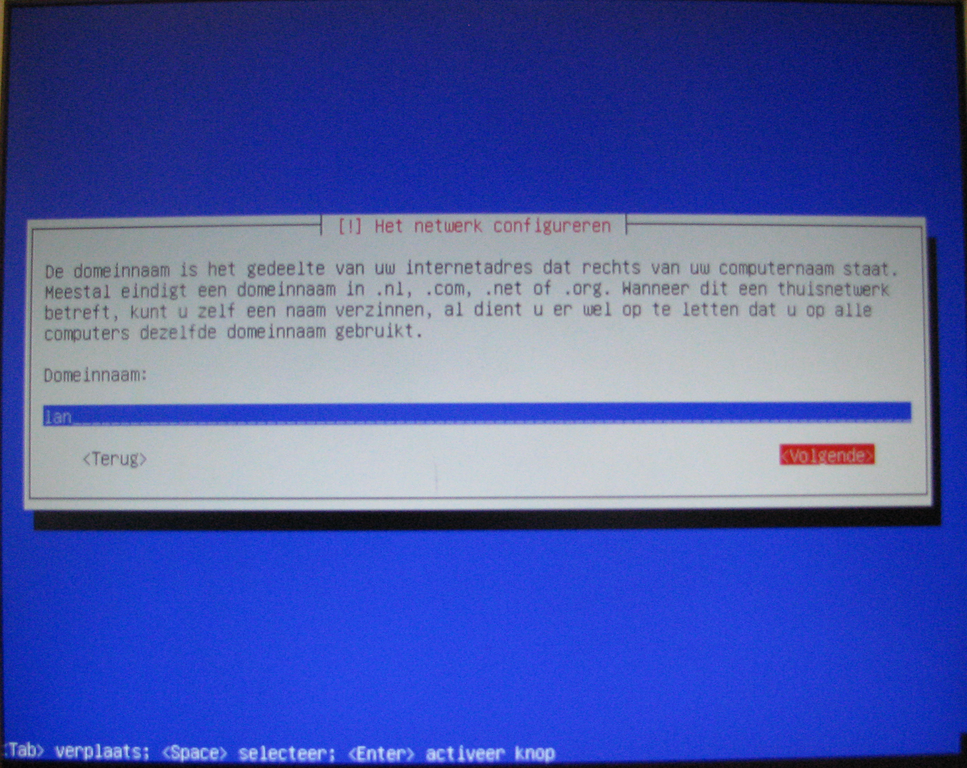
\includegraphics[width=0.45\textwidth]{domeinnaam-scherm}
\caption{Hostnaam en domeinnaam schermen.}
\label{fig:computernaam-scherm}
\end{figure}

Vul \textbf{debian} in als computernaam (figuur \ref{fig:computernaam-scherm}).

En vul \textbf{lan} in bij domeinnaam.


\subsection{Gebruikers en wachtwoorden}

\begin{figure}[H]
\centering
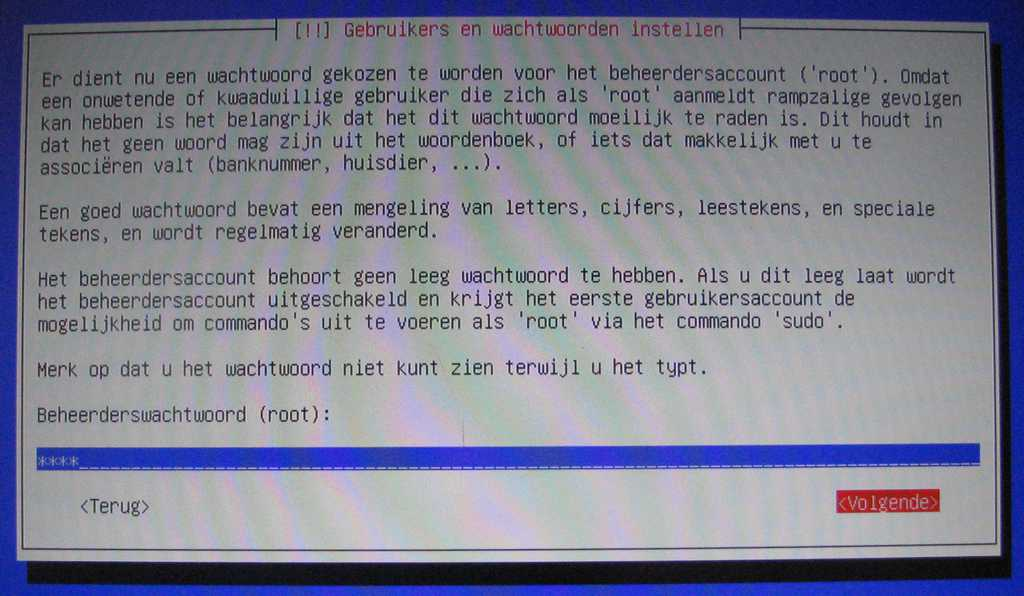
\includegraphics[width=0.45\textwidth]{root-wachtwoord-scherm}
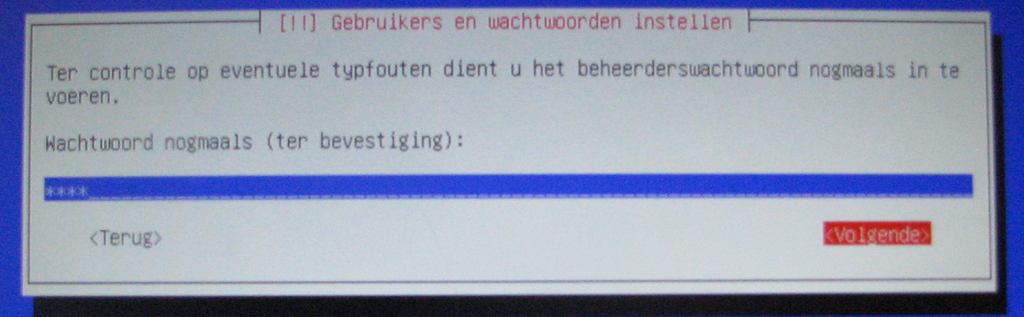
\includegraphics[width=0.45\textwidth]{root-wachtwoord-bevestiging}
\caption{Vul hier tweemaal \textbf{root} in.}
\label{fig:root-wachtwoord-scherm}
\end{figure}

Nu moeten het root wachtwoord worden gezet, zie figuur ~\ref{fig:root-wachtwoord-scherm}.
Vul als root wachtwoord in \textbf{root}, en doe dit nogmaals ter controle.

\begin{figure}[H]
\centering
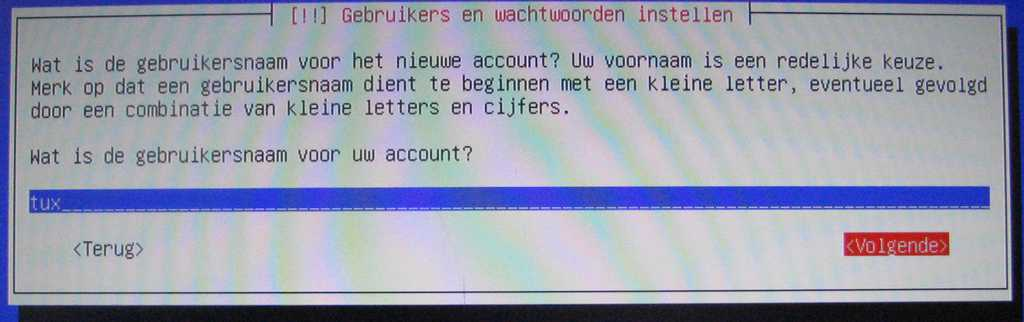
\includegraphics[width=0.45\textwidth]{nieuwe-gebruiker-naam}
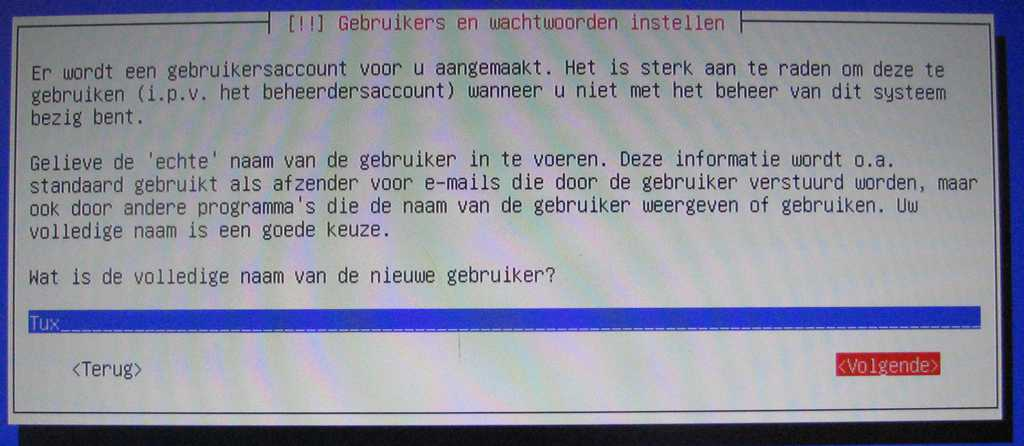
\includegraphics[width=0.45\textwidth]{nieuwe-gebruiker-echte-naam}
\caption{Toevoegen van een nieuwe gebruiker.}
\label{fig:nieuwe-gebruiker}
\end{figure}

Je vult \textbf{Tux} in als volledige naam van de nieuwe aardse gebruiker (figuur ~\ref{fig:nieuwe-gebruiker}).
De debian installer suggereert dan \textbf{tux} als gebruikersnaam.
Dat accepteer je met \textsc{enter}.

Als wachtwoord vul je \textbf{tux} in. Dit moet nog een keer worden bevestigd.


\subsection{Schijfindeling}
Bij de schijfindeling kies je \textbf{Begeleid - benut gehele schijf en gebruik LVM met encryptie}, zoals in figuur ~\ref{fig:schijven-indelen}.

\begin{figure}[H]
\centering
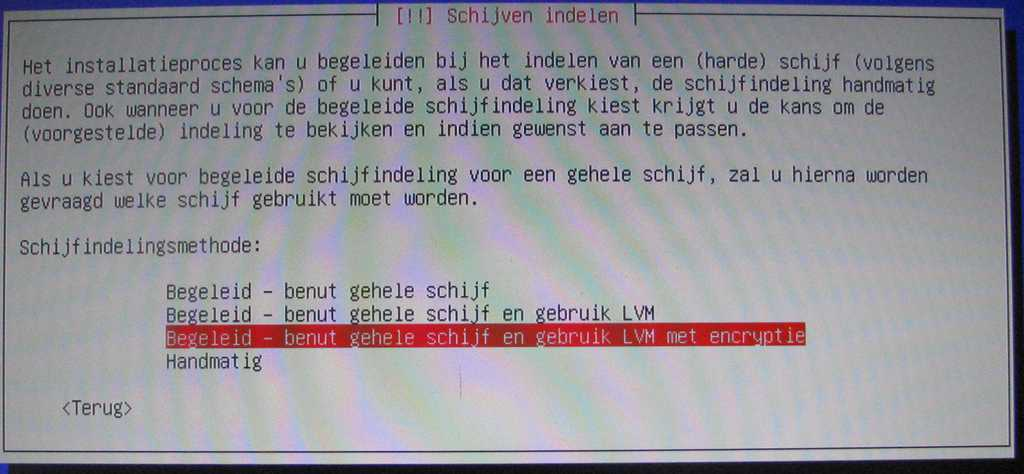
\includegraphics[width=0.45\textwidth]{schijven-indelen-scherm}
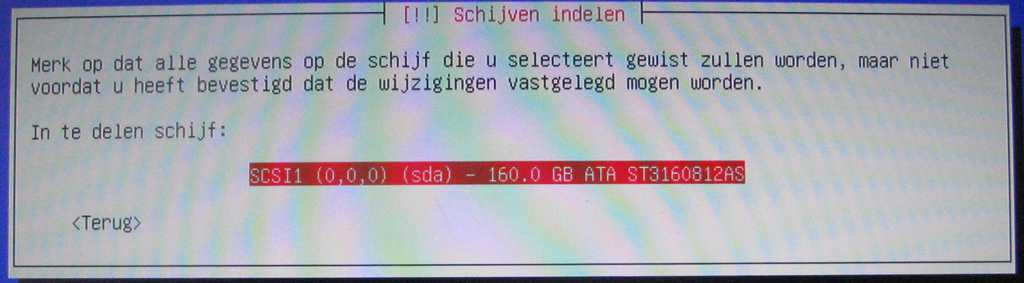
\includegraphics[width=0.45\textwidth]{schijf-uitkiezen-scherm}
\caption{Kies hier de optie met encryptie.}
\label{fig:ischijven-indelen}
\end{figure}



Nu moet je kiezen hoe de schijf gaat worden opgedeeld; je kiest de onderste optie \textbf{Afzondelijke /home, /usr, /var en /tmp partitie}.

Nu kies je de schijf die moet worden ingedeeld; dit zal meestal geen keuze opleveren, omdat de meeste machines maar \'{e}\'{e}n schijf hebben.

Nadat je dit bevestigd hebt, gaat de installer de gehele disk wissen, dat kan even duren (in de orde van uren). Je mag dit annuleren.

\begin{figure}[H]
\centering
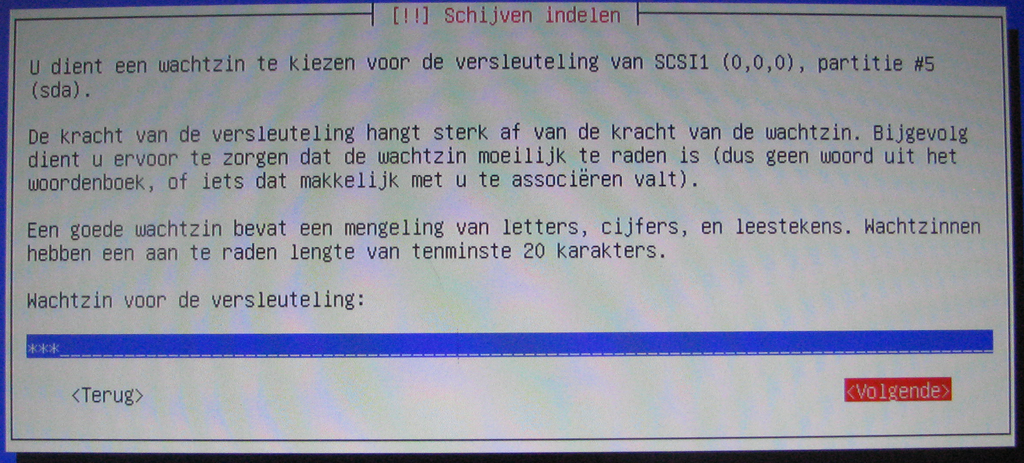
\includegraphics[width=0.45\textwidth]{schijven-wachtwoordzin-scherm}
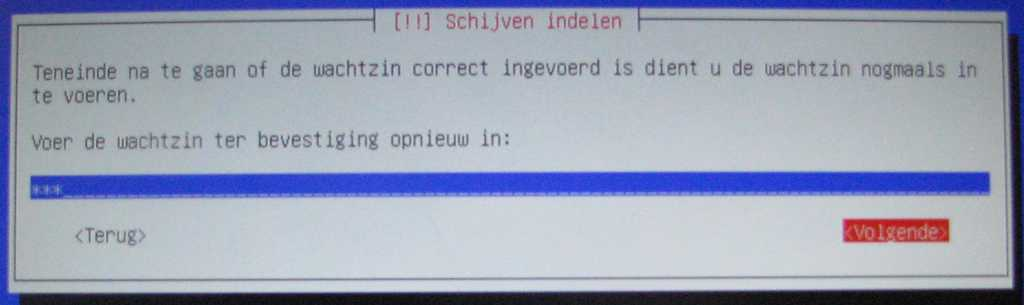
\includegraphics[width=0.45\textwidth]{schijven-wachtwoordzin-bevestiging}
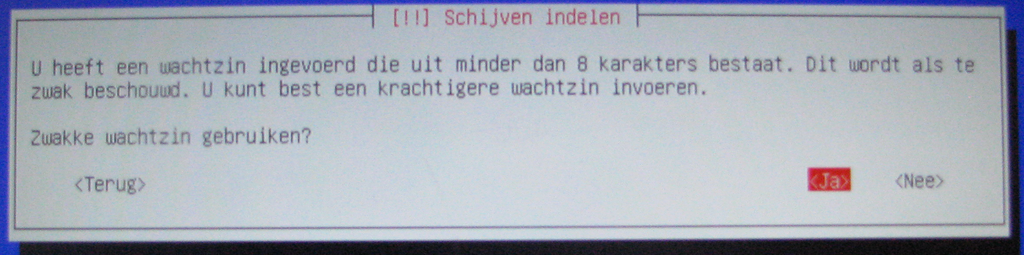
\includegraphics[width=0.45\textwidth]{schijven-zwakke-wachtwoordzin}
\caption{Kies hier de optie met encryptie.}
\label{fig:wachtwoordzin-scherm}
\end{figure}

Zoals in figuur ~\ref{fig:wachtwoordzin-scherm} wordt er om een wachtwoordzin gevraagd, je vult \textbf{gnu} in.

Dit moet je nogmaals te controle doen.

Je moet nu bevestigen dat dit een zwakke wachtwoordzin is. 

Het partitie schema wordt nog eenmaal aan je getoond opdat je het nog een keer kunt controleren. Je bevestigt de voorgestelde keuze.

\begin{lstlisting}[language=bash]
$lsof -i :80
\end{lstlisting}
Shows open files.
\end{document}
